\chapter{Forward Solutions}

\section{Overview}

As described previously, the solution to the forward problem deals with the calculation of the projection of properties from a source through some medium to set of collection locations.  In this application we will demonstrate, the forward problem specifically means the calculation of torso surface potentials from known cardiac source parameters.  There are two aspects of the forward problem that one must consider in order to solve it: how to model the source and how does that source map to the torso surface.  If presented as the classic $y=A(x)$,  with $y$ as the torso surface and $x$ as the cardiac source, choosing a model that is represented by $x$ is the source formulation.  $A$ is then dependent on the source model used must represent all relevant information about the torso geometry.

In regard to the source formulation, the two most common models are cardiac potentials and activation times.  The use of cardiac potentials is a more intuitive formulation in that the cardiac cells interact to change the extracellular potentials of the myocardium.  These potentials then project to the torso surface.  The activation time based source formulation deals with the nature that when there is inactive and active tissue next to each other, a source much like a dipole or layer of dipoles, is generated and that projects to the surface.  Both of these source models contain several assumptions, but each provides a generally accurate model that can be computationally reasonable.  

With the source formulation considered, one must now determine the pattern with which the source projects to the torso surface.  As mentioned, this relationship is dependent on the source model as well as the various properties of the torso, but in both source models presented the function $A$ can be represented by an $N \times M$ matrix, $N$ is the number of points on the cardiac surface and $M$ the number of points on the torso surface, which is called the lead field matrix.  Calculating this matrix can be a very computationally intensive task, and there are varying ways to do this.  The two examples given here find the lead field, or transfer matrix, are based on finite element method (FEM) and boundary element method (BEM).  The theory and mathematics behind these two methods are presented in Ch~\ref{sec:ch1}.

We provide here in this toolkit three methods to calculate the forward problem.  Potential based models using both FEM and BEM are demonstrated, as well as a activation time based model using FEM.  The BEM activation time forward problem is not yet supported in SCIRun, but it is performed in ECGSim, the interactive simulation software developed by Peacs in the Netherlands.\footnote{To obtain this free software, visit http://www.ecgsim.org/. Any references to ECGSIM herein are referring to version 1.3 beta}.  


An equivalent dipole layer is approximated as the source in the activation based forward problem.  


\section{Module Descriptions for Boundary Element Solutions}
The boundary element solution utilizes many common modules within the SCIRun framework
to read in files, visualize data, and manipulate geometry.  A descriptions of these modules
can be found in the SCIRun documentation whereas the modules that are relatively unique to the boundary element solution are outlined below.

SetFieldProperties is a module that allows you to define the conductivities inside a closed
surface as well as define the surface as a source or measurement surface.  For example, the heart with associated epicardial potentials, would be a source surface and the conductivity inside should
be set to 0.  While the torso surface, bones, and lungs would all be measurment surfaces and would 
each receive their own conductivity value.

\begin{figure}[H]
\begin{center}
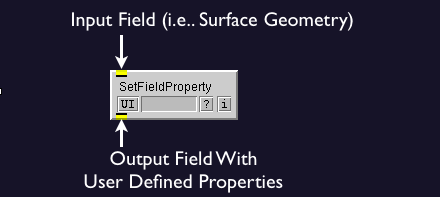
\includegraphics[width=12 cm]{ECGToolkitGuide_figures/SetFieldProps.png}
\caption{Module to set properties such as conductivity and if it is a source or boundary surface for the boundary element method}
\label{SetFieldProp}
\end{center}
\end{figure}

\begin{figure}[H]
\begin{center}
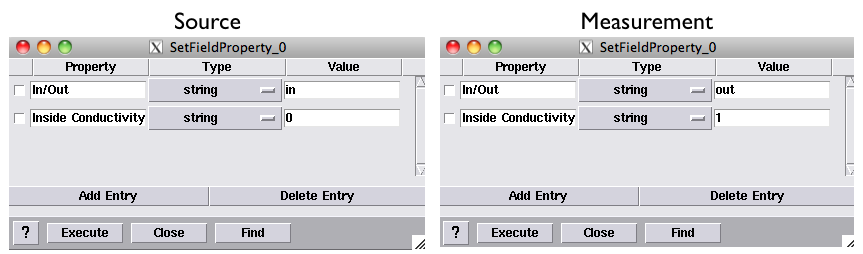
\includegraphics[width=\textwidth]{ECGToolkitGuide_figures/SetFieldPropGUI.png}
\caption{Shows the properties and values needed to create a source surface, left, or a 
measurement surface,right.}
\label{SetFieldPropGUI}
\end{center}
\end{figure}

After the properties have been set on the surfaces, they can be input into the BuildBEMatrix
module.  The first port takes the source surface and the module will dynamically add as many
additional ports as needed for the measurement surfaces.  The last surface input will be the surface
for which the transfer matrix projects the source potentials. 

\begin{figure}[H]
\begin{center}
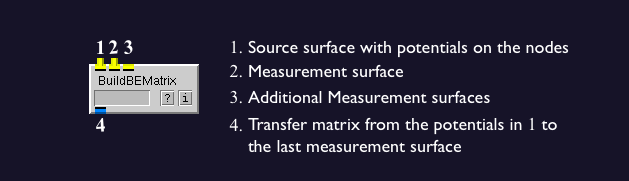
\includegraphics[width=\textwidth]{ECGToolkitGuide_figures/BEMmod.png}
\caption{Shows the module that computes the transfer matrix between the source surface
and the outermost measurement surface.}
\label{BEM}
\end{center}
\end{figure}

BuildBEMatrix assumes that for any closed surface, the surface normals will be pointing outward. The surface
normal for each element is determined using the node order from the connectivity definition of the mesh. The 
normals are defined using the right hand rule (counterclockwise) of the node order in each element. The 
module "FlipSurfaceNormals" can be used to flip all the element normals in the surface. It is important to check
the normals of the surfaces being used because incorrect normals will produce erroneous answers. 

\section{Module Descriptions for Finite Element Solutions}
The two most important modules for the forward finite element solution are the BuildFEMatrix 
and the AddKnownsToLinearSystem modules.  These allow you to compute a stiffness matrix and add boundary conditions.  The module BuildFEMatrix inputs a finite element mesh with the conductivities set on each element, or a lookup table may be used for the conductivities.  The result is a stiffness matrix based on the Galerkin method.

\begin{figure}[H]
\begin{center}
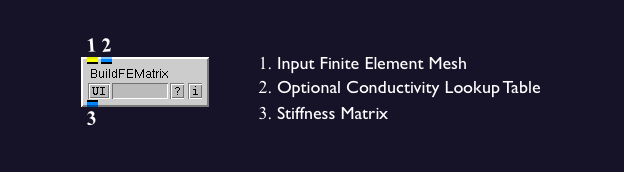
\includegraphics[width=\textwidth]{ECGToolkitGuide_figures/FEMmod.png}
\caption{Shows the module that computes the stiffness matrix for a FE solution.}
\label{FEM}
\end{center}
\end{figure}

AddKnownsToLinearSystem makes it possible to add known values as boundary conditions
to the linear system Ax=b.  Where A is the stiffness matrix, b is the right hand side vector, and 
x is known in the forward problem and unknown in the inverse problem.  The module must have stiffness matrix along with an x matrix.  If no right hand side matrix is provided, then it is assumed to be all zeros.  Know parameters are input along with the unknown values, while the unknown
values are set to 'nan'.

\begin{figure}[H]
\begin{center}
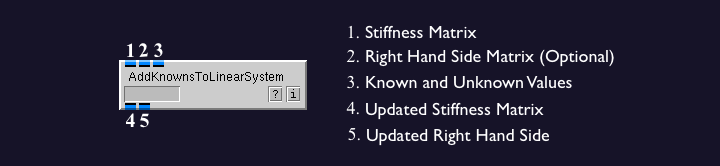
\includegraphics[width=\textwidth]{ECGToolkitGuide_figures/AddKnowns.png}
\caption{Shows the module that computes the stiffness matrix for a FE solution.}
\label{AddKnowns}
\end{center}
\end{figure}


\section{Example Networks for Boundary Element Solutions}
The following network shows the most basic implementation of the boundary element method
along with visualizing the results.  This networks reads in a epicardial surface mesh that has an associated matrix of epicardial potentials at each node.  The conductivities of the torso and heart
are set along with the differentiation between source and measurement surfaces in the SetFieldProperties module.  After which, a boundary element transfer matrix is computed and multiplied with the epicardial potentials.  This results in a torso potential field that can be visualized with SCIRun's ShowField module. 

\begin{figure}[H]
\begin{center}
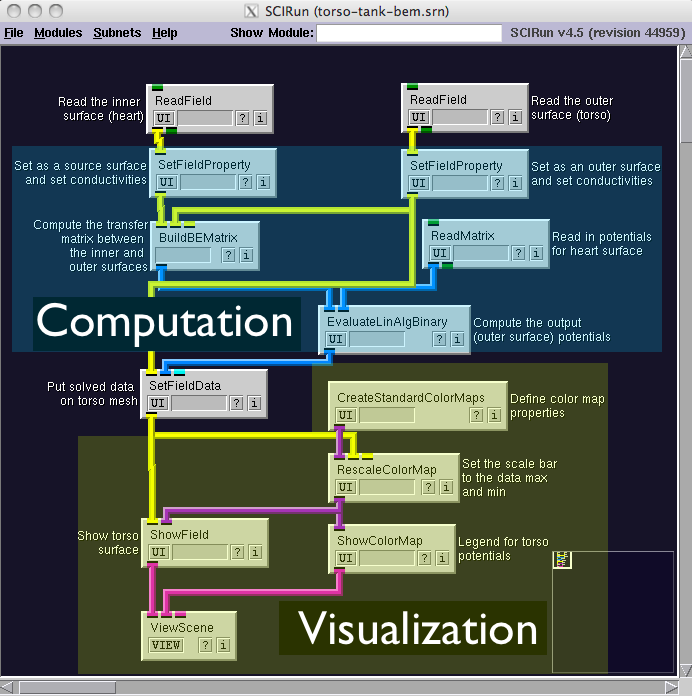
\includegraphics[width=\textwidth]{ECGToolkitGuide_figures/BEMnetwork.png}
\caption{Shows the implementation of the boundary element method.}
\label{BEMnet}
\end{center}
\end{figure}

\vspace{5pt}\textit{A similar SCIRun network for this example can be found at:\\``src/nets/FwdInvToolbox/potential-based-bem/torso-tank-bem.srn''\\in the SCIRun source code directory.}\vspace{5pt}

\section{Example Networks for Finite Element Solutions}

\subsection{Potential Based Forward FEM simulation}
\label{sec:pot_for_fem}

There are two examples given to calculate the potential based forward problem using finite element method.  One example involves the generation of the lead field matrix, or transfer matrix, then performing the forward calculation.  The other example is a direct calculation of the projection of the cardiac potentials onto the torso surface satisfying Laplace's equation.  

The inputs to the example networks in this section are all the same:  a torso segmentation, including segmentation of the heart volume, with a closed epicardium, a cardiac sock geometry registered to the heart volume from the segmentation, and a matrix of epicardial recordings that were obtained with an epicardial sock.  To calculate the lead field matrix, an identity matrix is also used for input vectors.

The example network {\tt potential-based-fem/forward\_problem.srn} provides an example of an easy implementation of the projection of the cardiac potentials onto the torso surface (Figure~\ref{fig:pot_for_fem}).  Though this problem is not formulated in the classic sense of the forward problem, it is useful because it does not require calculating the lead field matrix, which can take longer to compute in most cases.  This example presented is useful if a forward calculation requires a few time instances for a given geometry. Different time points may be selected in the {\tt GetColumnOrRowFromMatrix} module.

\begin{figure}[H]
\begin{center}
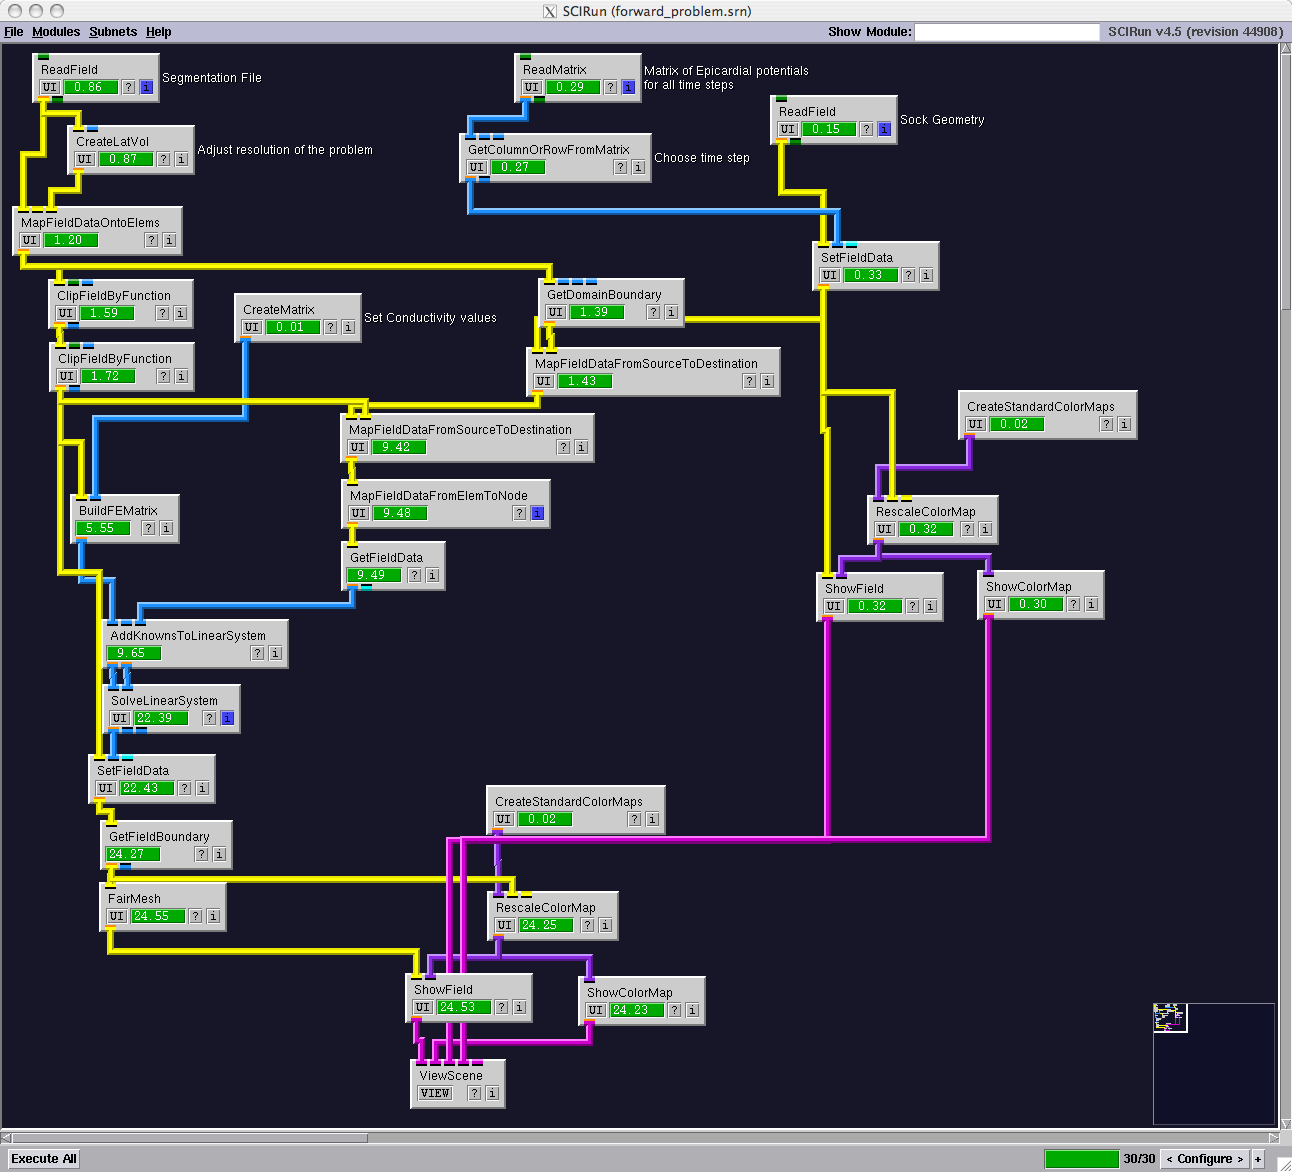
\includegraphics[width=\textwidth]{ECGToolkitGuide_figures/potential_forward_fem.png}
\caption{Simple potential based forward problem using FEM.}
\label{fig:pot_for_fem}
\end{center}
\end{figure} 

As mentioned above, the method implemented in this network uses Laplace's equation to find the torso potentials.  That is all the potentials in the torso satisfy the expression:
$$
\nabla \sigma \nabla \phi = 0
$$
where $\phi$ are the potentials and $\sigma$ are the conductivity values.  Using SCIRun, one is able to use the cardiac surface potentials as known values and solve the rest of the torso potentials to satisfy Laplace's equation as a linear system.

The example network {\tt potential-based-fem/forward\_problem\_with\_lead\_field\_matrix.srn} is a network that computes the forward problem in a more traditionally understood method (Figure~\ref{fig:pot_for_fem_w_mat}), in that it is a simple matrix multiplication to calculate the torso potentials.  This network simply uses a pre-computed lead field matrix and multiplies it by the cardiac potentials to yield the surface torso potentials.  Different time points may be selected in the {\tt GetColumnOrRowFromMatrix} module.

\begin{figure}[H]
\begin{center}
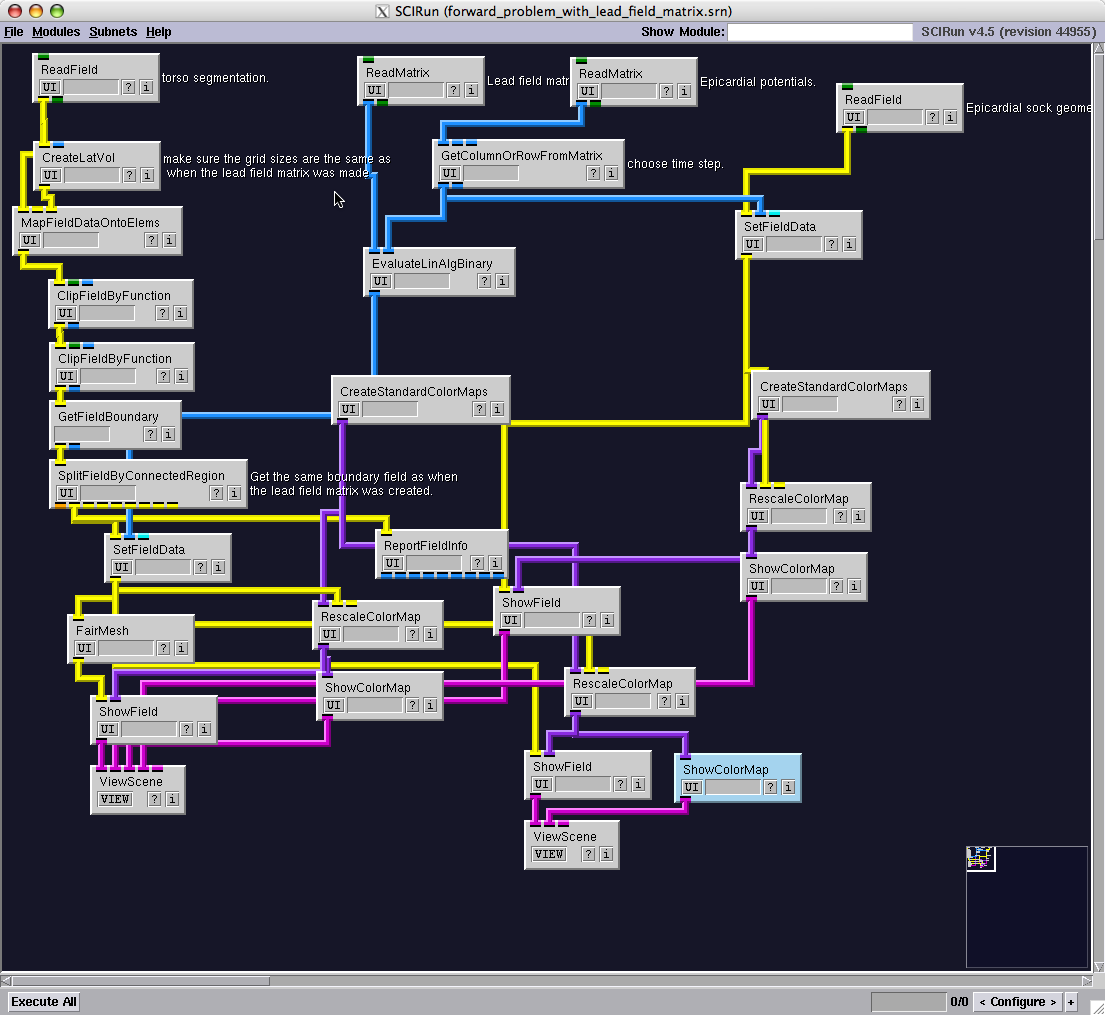
\includegraphics[width=\textwidth]{ECGToolkitGuide_figures/potential_forward_fem_with_leadfield.png}
\caption{Simple potential based forward problem using a pre-computed lead field matrix.}
\label{fig:pot_for_fem_w_mat}
\end{center}
\end{figure} 

The lead field matrix provided was generated by the network {\tt potential-based-fem/Make\_Lead\_field\_matrix.srn} (Figure~\ref{fig:mat_pot_fem}).  This network solves and collects the solution vectors relating isolated points on the heart to the torso.  The solution vector is calculated in the same manner as in the network {\tt potential-based-fem/forward\_problem.srn} described above using orthogonal unit vectors as the cardiac  potential (value of 1 at the point of interest and 0 elsewhere).  Computing the lead field matrix this way is very useful if there several forward calculations are needed on the same geometry.  

\begin{figure}[H]
\begin{center}
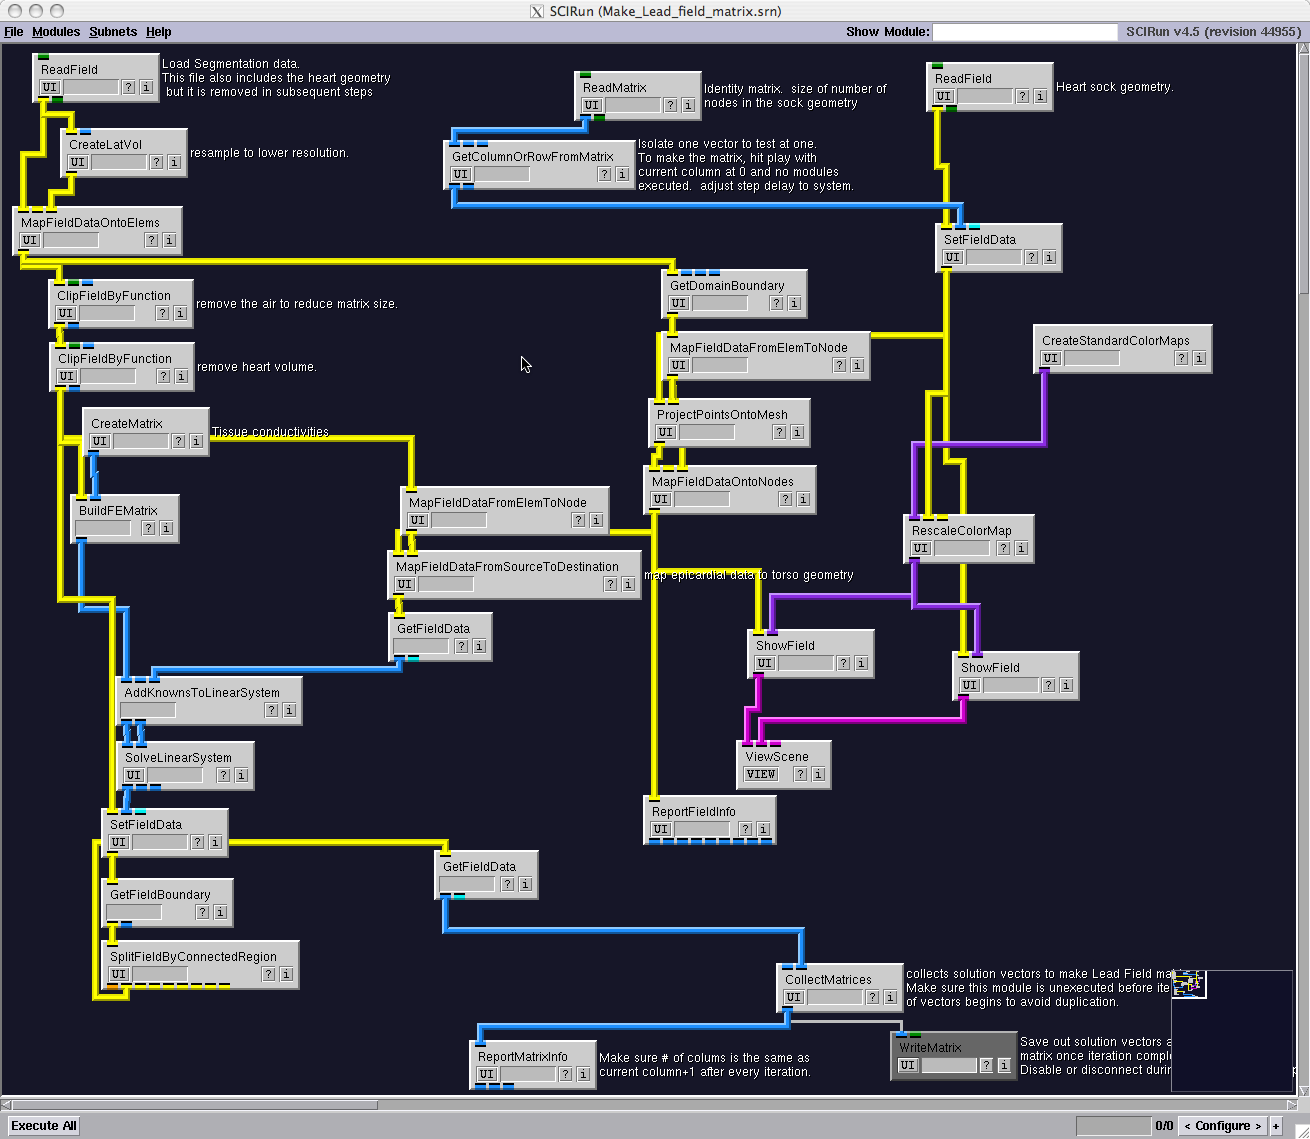
\includegraphics[width=\textwidth]{ECGToolkitGuide_figures/leadfield_pot_fem.png}
\caption{Computing the FEM based lead field matrix.}
\label{fig:mat_pot_fem}
\end{center}
\end{figure}

To calculate the lead field matrix with {\tt potential-based-fem/Make\_Lead\_field\_matrix.srn}:
\begin{enumerate}
\item{Make sure the {\tt CollectMatrices} module has not been executed.}
\item{Set step delay in the {\tt GetColumnOrRowFromMatrix} module is set to a sufficient interval so that all the modules can fully execute before the next iteration.}
\item{Set the current column to 0 and press play in the {\tt GetColumnOrRowFromMatrix}.}
\item{After the network finishes iterating, enable the {\tt WriteMatrix} module (by right clicking on the module), chose the place and name of the matrix you would like, and press save.  }
\end{enumerate}

\begin{figure}[H]
\begin{center}
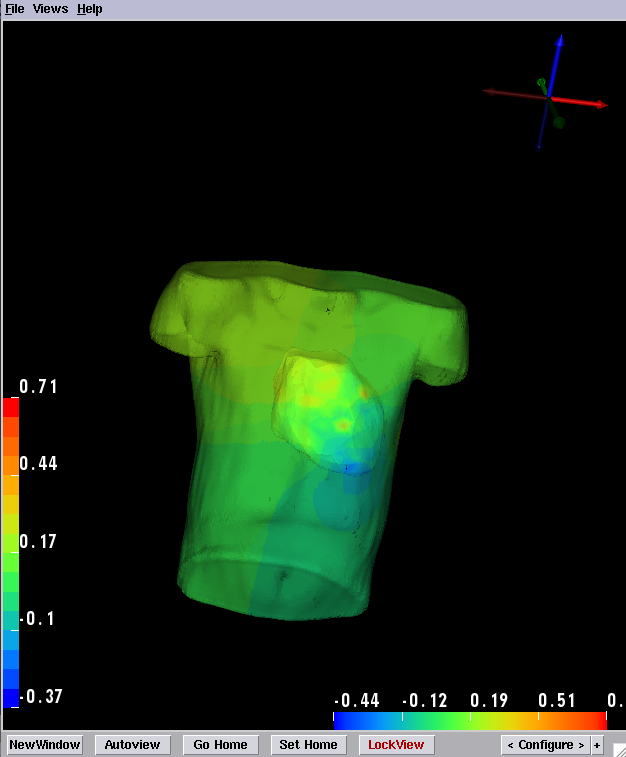
\includegraphics[width=\textwidth]{ECGToolkitGuide_figures/pot_fem_forward_output.png}
\caption{Solution of the potential based forward problem using FEM.}
\label{fig:pot_fem_for_sol}
\end{center}
\end{figure}
 


\subsection{Activation Based Forward FEM simulation}

The technique used in the activation based model is to specify whether
or not each region of the heart surface is ``active'' and what the
activation profile looks like at each node of a surface representing
the heart. This is very different than the activation profile on a
cellular level as each surface node represents a large region of the
heart. The activation profile is used to specify the strength of
dipoles located on the surface.  This source formulation is 

As FEM is a volume method, SCIRun approximates these dipoles by
clipping the volume mesh with the surface mesh used to specify the
activation profile, giving a volume mesh that roughly follows the
surface mesh. The potentials on the outer and inner boundaries of this
volume mesh are set to approximate dipoles at the heart surface.

There are three networks located in {\tt   activation-based-fem} 
which provide an example of activation based forward calculation 
using FEM.   The three networks are similar in nature the potential
 based FEM forward problem networks explained in Sec.~\ref{sec:pot_for_fem}.
 The activation based forward problem networks use data derived from ECGSIM
  The surface mesh and source
parameters are also obtained from the ECGSIM project.

The primary inputs to this network are the surface mesh representing
the heart, a torso surface mesh, which is made a volume mesh 
(refined near the surface of the heart) in the network, and
a matrix specifying the activation profile for each point in the heart
surface mesh at each time to be simulated. This matrix is then of size
$N \times M$ where $N$ is the number of surface points and $M$ is the
number of time-steps represented. A very good example of the input
expected can be obtained from the ECGSIM software by choosing {\em
  Save $\rightarrow$ Source parameters} from the {\em File} menu.
  
Though the {\tt activation-based-fem.srn} networks seem quite complicated, it performs some simple tasks.  The loaded torso surface is made into a volume and refined in nearer to the heart.  Then two cardiac surfaces are made from the first, one slightly inside, one slightly outside the heart.  The corresponding points on the two surfaces are set to either active, or inactive.  If the point is inactive, then it is set as an unknown and will be solved for later.  If the point is active, the two surfaces are set to opposing values to approximate a dipole layer.  The remaining torso potentials are solved using a linear systems solver similar to Sec.~\ref{sec:pot_for_fem}.
  
The network {\tt activation-based-fem\_lead\_field.srn} produces similar results as the previous network, but it utilizes a pre-computed lead field matrix.  This network allows for the activation times to be directly related to the torso surface and the computation is relatively quick.  This method is also more like the traditionally formulated forward problem with a simple matrix multiply.

The lead field matrix is calculated using the  {\tt make\_lead\_field.srn} network.  Similar to potential based approach (Sec.~\ref{sec:pot_for_fem}), the solution vectors for each point on the cardiac surface are calculated and collected as the lead field matrix.  This is essentially a pre-computation of the contribution of each point.  This calculation is very useful if the geometry is going to be used many times.
  
  
  To calculate the lead field matrix with {\tt make\_lead\_field.srn}:
\begin{enumerate}
\item{Make sure the {\tt CollectMatrices} module has not been executed.}
\item{Set step delay in the {\tt GetColumnOrRowFromMatrix} module is set to a sufficient interval so that all the modules can fully execute before the next iteration.}
\item{Set the current column to 0 and press play in the {\tt GetColumnOrRowFromMatrix}.}
\item{After the network finishes iterating, enable the {\tt WriteMatrix} module (by right clicking on the module), chose the place and name of the matrix you would like, and press save.  }
\end{enumerate}

\begin{figure}[H]
\begin{center}
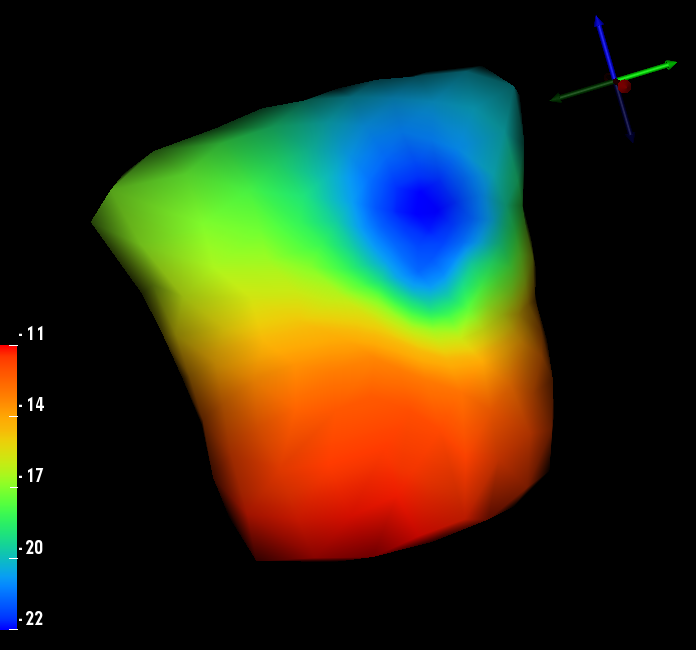
\includegraphics[width=\textwidth]{ECGToolkitGuide_figures/act_for_fem_results.png}
\caption{Solution of the activation based forward problem using FEM.}
\label{fig:act_fem_for_sol}
\end{center}
\end{figure}

